\documentclass[twocolumn,norwegian]{article}
\usepackage{hyperref}
\hypersetup{colorlinks=true}
\usepackage{titling}
\usepackage{algorithmic}
\usepackage{algorithm}
\usepackage{graphicx}
\usepackage{amsmath}
\usepackage[caption=false,font=footnotesize,labelfont=bf,textfont=sf]{subfig}
\usepackage[labelfont=bf, font=small]{caption}
\usepackage{multirow}
\usepackage{arydshln}
\graphicspath{{figures/}}

%\usepackage[showframe]{geometry}
\usepackage{layout}
\setlength{\voffset}{-0.6in}
\setlength{\hoffset}{-0.35in}
\setlength{\textwidth}{480pt}
\setlength{\textheight}{620pt}

%\setlength{\droptitle}{-1cm} 

%opening
\title{TEK9020 - Prosjektoppgave 3}
\author{Kristoffer Langstad \\ kristoffer.langstad@its.uio.no}
\date{}

\begin{document}%\layout
	
	\maketitle
	
	\section{Introduksjon}
	I denne oppgaven er målet å se hvordan forskjellige metoder for klyngeanalyse fordeler samplene i et datasett til ulike klasser utifra egenskapene til samplene, for så å evaluere klyngene med noen standard klassifikatorer. Klyngeanalyse brukes ofte i ikke-ledet læring sammenhenger for å fordele samplene i datasett inn i klasser for å gi en bedre oversikt og kunnskap om datasettet. I dette tilfellet brukes Fisher's Iris blomster datasett, som inneholder kjente klasser. De kjente klassene brukes for evaluering sin skyld, der det fokuseres på det ikke-ledet læring tilfellet med klyngeanalyse. Det skal ses på to forskjellige klyngemetoder, KMeans og agglomerativ metode, for å dele samplene i Iris datasettet inn i klynger. Så vil disse klyngemetodene evalueres opp mot de sanne klassene, og ses på forskjeller mellom metodene.
	
	Først presenteres litt teori om klyngeanalyse og de to klyngemetodene, så presenteres datasettet, etterfulgt av metodikken med eksperimenter og hvilke klassifikatorer som skal brukes. Resultater og diskusjoner av resultatene blir så presentert til slutt med en liten konklusjon av oppgaven. Programmeringen er utført i Python~(\ref{Appendix:Kode}).

	
	\section{Teori - klyngeanalyse}
	Det sentrale i klyngeanalyse er å dele inn samplene i datasett inn i klynger utifra likheter i egenskapene til samplene. Samplene med mest mulig like egenskaper fordeles i klynger, samtidig mens det er størst mulig ulikhet til andre sampler. For slike tilfeller er det som oftest ikke kjent klassetilhørighet, ikke-ledet læring, slik at klyngeinndelingene kun baseres på egenskapvektorene til samplene, og ikke a priori kunnskap. På denne måten få kunnskap om strukturer i data som ellers ofte er ukjent. Disse lagde klyngene kan så brukes til videre analyse, der det kan antas at hver klynge tilsvarer hver sin klasse. I tilfeller der datasettet kan merkes utifra klyngene, så kan det brukes til ledet læring ved å trene klassifikatorer.

	For å dele samplene inn i klynger med like egenskaper, brukes en avstandsmåler.
	Denne avstanden spiller en viktig rolle i hvordan datasettet blir fordelt. En av de mest vanlige metrikkene er Euklidsk avstand:
	\begin{equation}
		\label{eq:Euclidsk avstand}
		d(\textbf{x}_1, \textbf{x}_2) = ||\textbf{x}_1 - \textbf{x}_2||
	\end{equation}
	Utifra avstanden mellom to sampler, kan det da settes kriterier for hvilke sampler som skal i samme klynge. Det enkleste er oftest å fordele sampler i samme klynge dersom den Euklidske avstand er mindre enn en satt verdi. F.eks. at sample $\textbf{x}_1$ og sample $\textbf{x}_2$ er i samme klynge dersom $d(\textbf{x}_1, \textbf{x}_2)<d_0$. Det vil da være klynger der innbyrdes avstand er liten mellom sampler, sammenlignet med sampler i andre klynger. 
	
	Det er flere slike klyngemetoder, men det skal fokuseres på KMeans clustering og en hierarkisk metode i dette prosjektet.
	
	
	\subsection{KMeans clustering}
	Den første metoden i bruk er KMeans clustering. Dette er en slags topp-ned metode som er basert på å lage klyngesenter og iterativt fordele samplene til nærmeste klynge med hjelp av en distanse metode, samtidig som klyngesentrene oppdateres underveis. Distanse metoden måler avstanden mellom de ulike samplene og klyngene for å iterativt tilegne samplene til $k$ gitte klynger. Iterasjonsprosessen er lignende som Algoritme~\ref{alg:KMeans}.
	\begin{algorithm}
		\caption{KMeans iterasjonsprosess.}
		\label{alg:KMeans}
		\begin{algorithmic}
			\STATE *Initialisér $\hat{\mu}_1$, ..., $\hat{\mu}_c$
			\STATE *Gjenta inntil ferdig:
				\STATE \quad -Klassifiser $x_k$, k=1, ..., n til nærmeste senteroide ved hjelp av Euclidsk avstand
				\STATE \quad -Oppdater $\hat{\mu}_1$, ..., $\hat{\mu}_c$
				\STATE \quad -Hvis ingen endring $\rightarrow$ ferdig
		\end{algorithmic}
	\end{algorithm}
	
	Ulemper: En mulig ulempe med KMeans metoden er at den krever en viss a prior kunnskap om datasettet, nemlig antall klasser/klynger datasettet skal deles inn i. Dersom dette er ukjent informasjon, så finnes det metoder for å få mer informasjon som kan tilnærme seg hva som er riktig antall klynger. En slik metode er Albue metoden (Eng: Elbow method), der det regnes ut og plottes ''within-cluster sum of squares'' (WCSS) mot antall klynger. WCSS beregner den kvadratiske avstanden mellom hvert sample og senteroiden dens. Albue metoden produserer en kurve lik som Figur~\ref{fig:Elbow}, som er lagd til dette prosjektet på Iris datasettet for å vise den optimale mengden klynger, som her er 3 både utifra kurven og siden dette er kjent for oss med 3 klasser. Det optimale antall klynger finnes i knekken på kurven der kurven ikke lenger endrer seg betraktelig, som passer for 3 klynger.
	\begin{figure}[ht!]
		\centering
		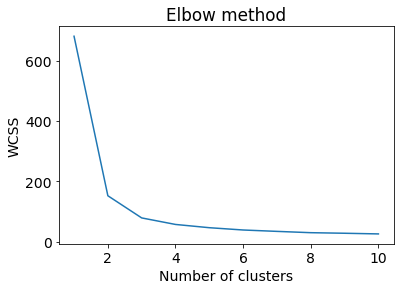
\includegraphics[width=\linewidth]{KMeans_class/Elbow.png}
		\caption{Albue metoden for å finne optimalt antall klynger for et gitt datasett. Her brukt på Iris datasettet.}
		\label{fig:Elbow}
	\end{figure}
	
	
	\subsection{Hierakiske metoder}
	Det er flere hierarkiske metoder brukt innen klyngeanalyse, men det fokuseres på den agglomerative metoden. Den agglomerative metoden fungerer som en bunnen-opp metode der hvert sample er hver sin klynge til å begynne med. Deretter brukes en avstands måler, ofte Euklidsk avstand, for å slå sammen de to nærmeste klyngene hvert steg. Dette fortsetter til alle klyngene har blitt slått sammen til en stor klynge. Den agglomerative metoden kan ses i Algoritme~\ref{alg:Agglo}.
	\begin{algorithm}
		\caption{Agglomerativ iterasjonsprosess.}
		\label{alg:Agglo}
		\begin{algorithmic}
			\STATE *Start med $k$ klynger, dvs. $\chi_i$=$\{x_i\}$, i=1, ..., c; $\hat{c}=k$
			\STATE *Finn nærmeste par av klynger, f.eks. $\chi_i$, $\chi_j$
			\STATE *Slå sammen disse klyngene $\hat{c}\rightarrow \hat{c}-1$ 
			\STATE *Gjenta de to forrige trinnene til antall ønsket klynger $\hat{c}=c$ er funnet.
		\end{algorithmic}
	\end{algorithm}
	
	Så lages et Dendrogram som i Figur~\ref{fig:Dendrogram}, denne figuren kan minne om et tre med røtter, der kan det ses utifra figuren hvilket antall klynger det kan være i datasettet. Antall klynger kan bestemmes ut ifra høyden mellom stegene/avstanden. Dendrogrammet i Figur~\ref{fig:Dendrogram} er lagd på Iris datasettet, og viser stor avstand når den har kommet til 3 klynger, som stemmer bra med det som er kjent om datasettet med 3 klasser.
	\begin{figure*}[t!]
		\centering
		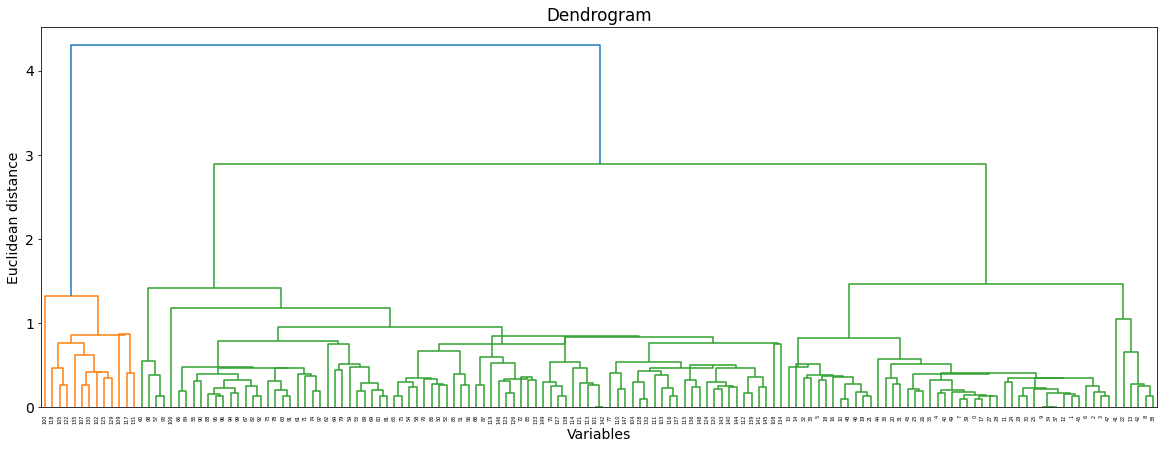
\includegraphics[width=1\linewidth,height=0.23\textheight]{Agglomerative_class/Dendrogram.png}
		\caption{Dendrogam lagd på Iris datasettet for å finne optimalt antall klynger.}
		\label{fig:Dendrogram}
	\end{figure*}
	
	
	\section{Metode}
	Her ses det kort på hva Iris datasettet inneholder, før selve eksperimentene forklares for å produsere resultatene.
	
	\subsection{Datasett}
	Datasettet som brukes i dette prosjektet er et mye brukt datasett innen mønstergjenkjenning som heter Iris. Fisher's Iris datasett inneholder tre typer varianter av iris blomster (Setosa, Versicolor, Virginica) med 50 sampler hver, i tillegg til at hver sample har fire egenskaper relatert til lengde og bredde på begerbladene og kronbladene:
	\begin{itemize}
		\item SepalLengthCm
		\item SepalWidthCm
		\item PetalLengthCm
		\item PetalWidthCm
	\end{itemize}
	Alle blomstene er variasjoner av Iris blomsten, der to av typene er fra samme område og tidspunkt, som gjør at to av blomstene har likere egenskaper men fortsatt ulike hverandre.

	Datasettet inneholder også de sanne klassene til blomstene. For å bruke dette datasettet til ikke-ledet læring og klyngeanalyse så utelates de sanne klassene fra datasettet for KMeans og agglomerativ klyngemetoder.
	
	
	\subsection{Eksperimenter}
	Dette prosjektet kan deles inn i tre eksperimenter: Først se hvordan det originale Iris datasettet ser ut i klynger og hvordan noen standard klassifikatorer klarer å trene og klassifisere datasettet. Nummer to er å bruke KMeans metoden for å tildele datasettet, uten klasser, inn i nye klynger, og se hvordan klassifikatorene gjør det på disse klyngene. Nummer tre er å bruke agglomerativ metode for å lage klynger og gjøre samme analyse som for KMeans metoden.
	
	Med det originale Iris datasettet med klassene tilgjengelige, visualiseres enkelt de tre blomster klynge egenskapkombinasjonene i en samlet figur, i et såkalt par-plot. For KMeans og agglomerativ metode, så brukes albue metoden og dendrogram for å vise at antall klasser i datasettet er tre. Så må de først dele samplene inn i klynger, som er uten kjent klassetilhørighet. Dette gjør at de produserte klyngene i utgangspunktet ikke er markerte med klasse, men for visualisering og sammenlignbarhet, så brukes de kjente klassetilhørighetene for å vise med navn hva de forskjellige klyngene er. Å legge til klassenavnene gjøres manuelt for de visualiseres.
	
	Etter at klyngene har blitt produsert med de to klyngemetodene, så brukes de kjente klassene for å evaluere hvor nøyaktige de to metodene er sammenlignet med de originale klyngene. Deretter brukes klassifikatorene til å trene og predikere sampler inn i riktige klynger, som kan sammenlignes mellom de tre klyngene som er lagd og  visualisert.
	
	Siden klyngemetodene er statistiske metoder, hjelper det ofte å involvere kryssvalidering og ta gjennomsnitt av prediksjonene. Dette er for å være sikker på at ikke resultatene bare er avhengige av kun en prediksjon, der noe av dataen kanskje utelates fra analysen. Dette er med tanke på å dele datasettet inn i trening og test sett, f.eks. 80\% trening og 20\% testing. Med kryssvalidering sørges det for at for hver kryssvalidering så endres hvilke sampler som blir en del av test settet. Derfor utføres kryssvalidering 5 ganger for hver klassifikator for å gi endelig evaluering.
	
	
	\subsubsection{Klassifikatorer}
	For å bruke klassifikatorene til å evaluere klyngemetodene, så brukes det at klassene er kjente for å bruke ledet-læring klassifisering. Klassifikatorene som brukes i dette prosjektet er:
	\begin{itemize}
		\item K-Nærmeste Nabo (Eng: K-Nearest Neighbors, KNN): Fordeler sampler inn i klasser basert på likheter i egenskapene til samplene.
		\item Logistisk regresjon (Eng: Logistic regression, LR): Den bruker sannsynlighet for å bestemme hvilken klasse et sample tilhører.
		\item Støttevektormaskiner (Eng: Support Vector Machine, SVM): Prøver å finne det hyperplanet som best mulig separerer samplene i klasser.
		\item Beslutningstrær: Bruker trestrukturer for å tildele et sample til en klasse utifra flere spørsmål eller kriterier. Dette kan være et enkelt tre (Eng: Decision Tree, DT), eller det kan brukes sammensetninger av flere trær (Eng: Random Forest, RF).
		\item Nevrale nettverk (Eng: Neural network, NN): Bruker opptil flere lag med nevroner som samarbeider om å lære mønstre i data, som så brukes til å predikere klasser. Bruker her en enkel Multi-layer perceptron model (MLP).
	\end{itemize}
	
	For å evaluere klassifikatorene, brukes hovedsaklig hvor nøyaktige prediksjonene er sammenlignet med de sanne klassene (accuracy score), og forvirringsmatriser (confusion matrix) som viser antall riktige og ikke riktige gjetninger per klasse.
	
	
	\section{Resultater}
	Presenterer her noen av resultatene som er produsert som brukes for å sammenligne klyngene og metodene. Andre resultater som er produsert, i tillegg til de som vises her, kan ses ved å følge GitHub-linken i~\ref{Appendix:Kode}.
	
	
	\subsection{Klynge-inndelinger}
	I Figur~\ref{fig:Datasett} vises for en kombinasjon med to av egenskapene, fra venstre; de originale Iris klyngene~(\ref{subfig:Orig_klynge}), klyngene som er lagd med KMeans metoden~(\ref{subfig:KMean_klynge}), og klyngene som er lagd med agglomerativ metode~(\ref{subfig:Agglo_klynge}). Dette er en av egenskapkombinasjonene for å vise klyngene for de tre tilfellene. I Figur~\ref{fig:Pairplot} vises alle egenskapkombinasjonene for å vise hvordan kombinasjoner av egenskapene til Iris datasettet kan brukes for å vise samplene. I visse tilfeller er det enklere å skille to av klassene, mens for andre kombinasjoner er det mer overlapp mellom samplene. Egenskapkombinasjonen i Figur~\ref{fig:Datasett}, er en av de med mest overlapp for Iris-versicolor og Iris-virginica klassene.
	
	I Figur~\ref{fig:Klynger_confmat} vises forvirringsmatrisene lagd av KMeans og agglomerativ metode på Iris datasettet, uten kjente klasser, sammenlignet med de sanne klassene i Iris datasettet for å se hvilke klasser de to klyngemetodene predikerer bra.
	
	\begin{figure}[h!]
		\vspace{-0.1cm}
		\centering
		\subfloat[Original]{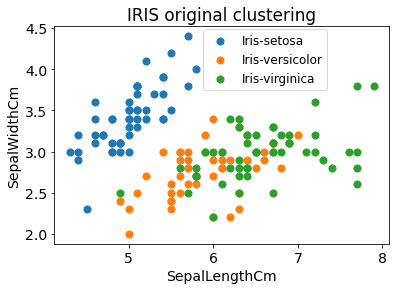
\includegraphics[width=0.33\linewidth]{Original_class/IRIS original clustering.png}
			\label{subfig:Orig_klynge}}
		\subfloat[KMeans]{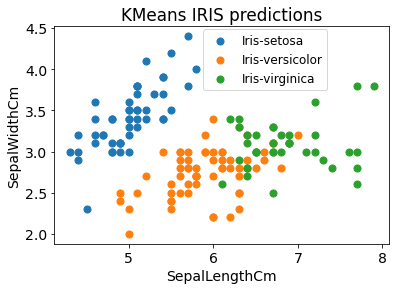
\includegraphics[width=0.33\linewidth]{KMeans_class/KMeans IRIS predictions.png}
			\label{subfig:KMean_klynge}}
		\subfloat[Agglomerativ]{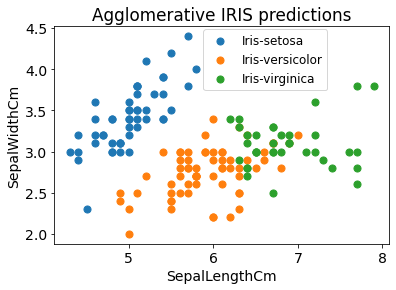
\includegraphics[width=0.33\linewidth]{Agglomerative_class/Agglomerative IRIS predictions.png}
			\label{subfig:Agglo_klynge}}
		\caption{Fra venstre: Klyngeinndelinger for det originale Iris datasettet~(\ref{subfig:Orig_klynge}), klynger lagd med KMeans metode~(\ref{subfig:KMean_klynge}), og klynger lagd med agglomerativ metode~(\ref{subfig:Agglo_klynge}). \label{fig:Datasett}}
	\end{figure}
	\begin{figure}[hb!]
		\vspace{-0.4cm}
		\centering
		\subfloat{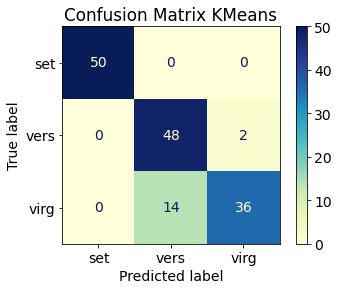
\includegraphics[width=0.5\linewidth]{KMeans_class/KMeansconfmat.png}}
		\subfloat{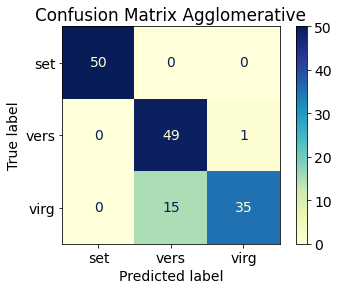
\includegraphics[width=0.5\linewidth]{Agglomerative_class/Agglomerativeconfmat.png}}
		\caption{Forvirringsmatriser for KMeans og agglomerativ metode.}
		\label{fig:Klynger_confmat}
	\end{figure}
	
	\begin{figure}[h!]
		\centering
		\subfloat{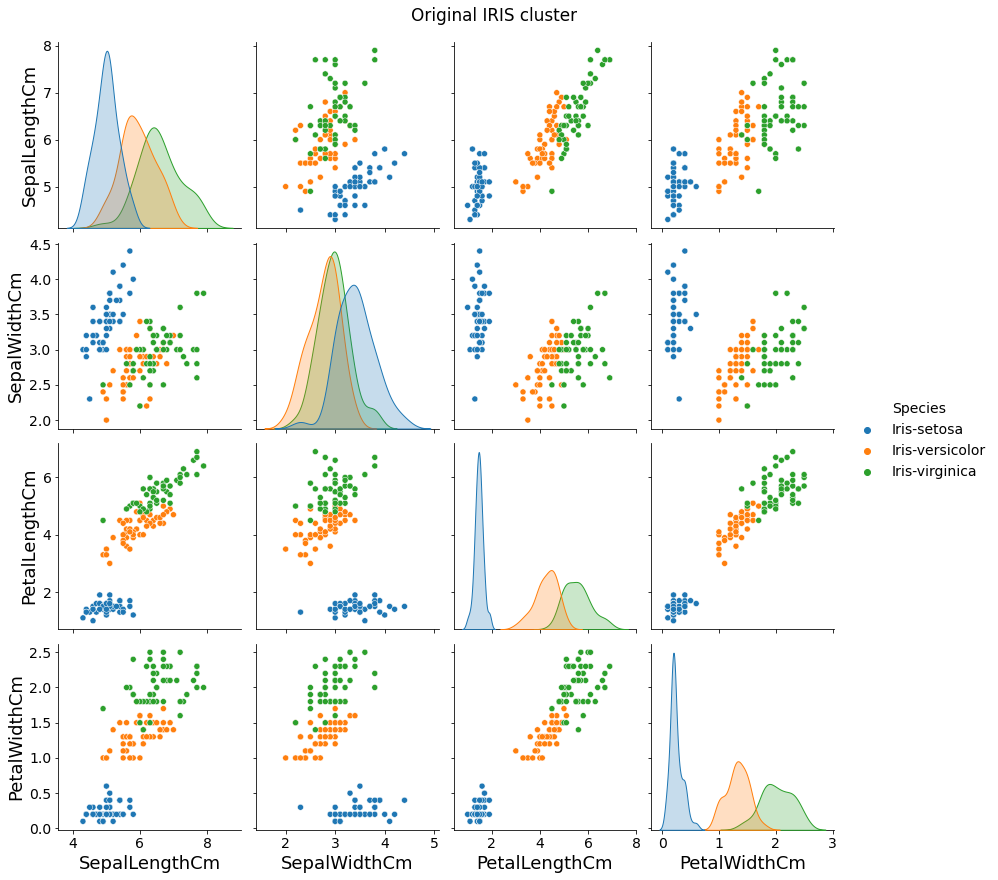
\includegraphics[width=0.89\linewidth]{Original_class/Original cluster.png}}\\
		\subfloat{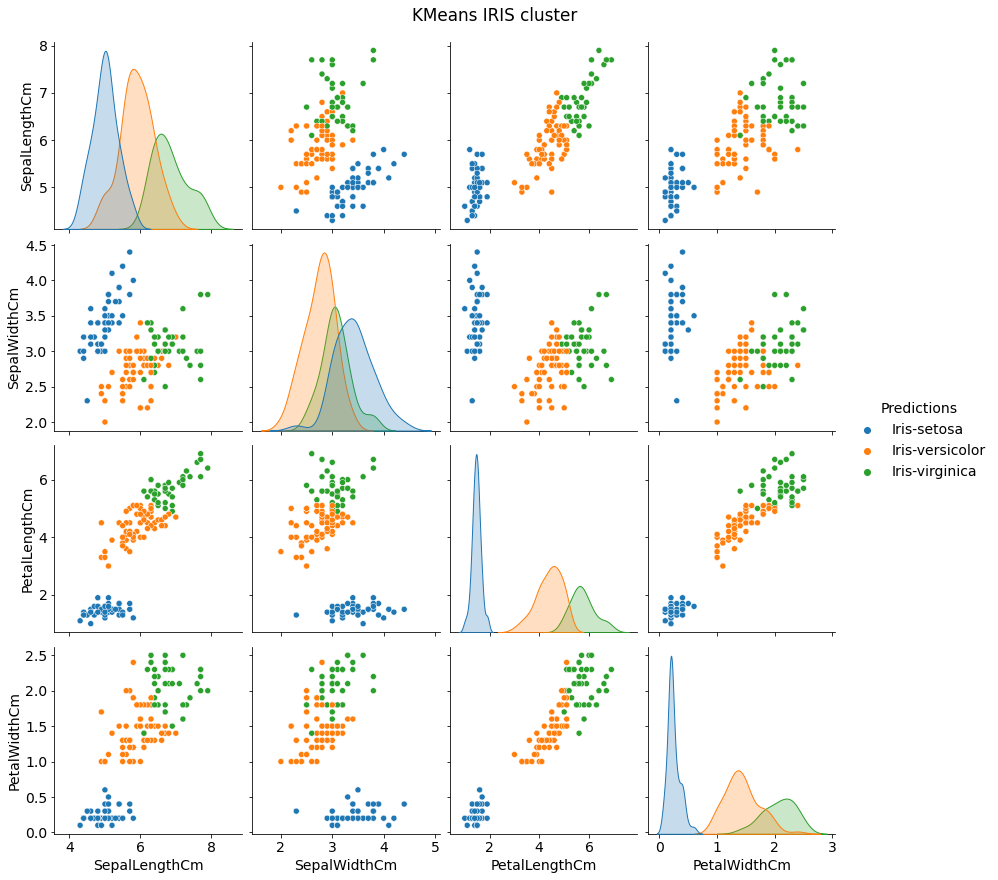
\includegraphics[width=0.89\linewidth]{KMeans_class/KMeans.png}}\\\
		\subfloat{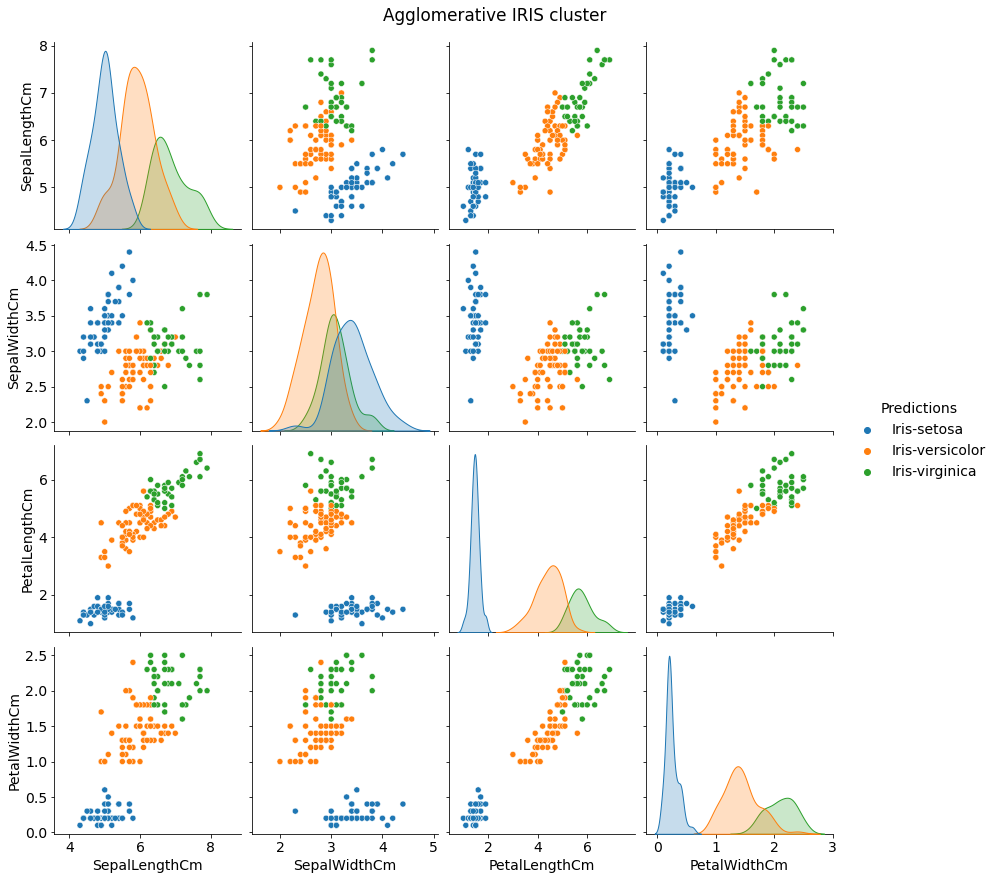
\includegraphics[width=0.89\linewidth]{Agglomerative_class/Agglomerative.png}}
		\caption{Alle parvis egenskapkombinasjoner for de tre klynge tilfellene.}
		\label{fig:Pairplot}
	\end{figure}
	
	

	\begin{figure*}[t!]
		%\vspace{-0.2cm}
		\centering
		\subfloat{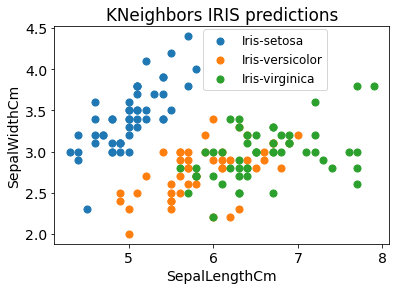
\includegraphics[width=0.26\linewidth]{Original_class/KNeighbors IRIS predictions.png}}
		\subfloat{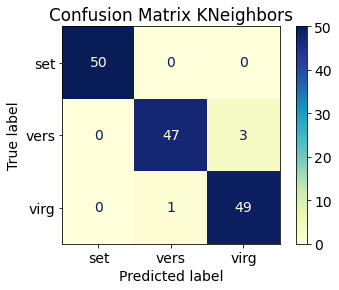
\includegraphics[width=0.23\linewidth]{Original_class/KNeighborsconfmat.png}}
		\subfloat{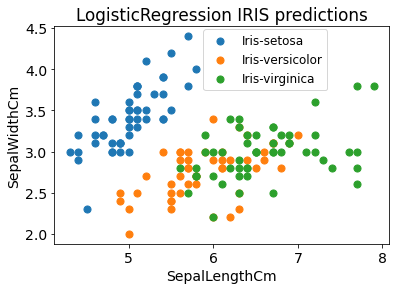
\includegraphics[width=0.26\linewidth]{Original_class/LogisticRegression IRIS predictions.png}}
		\subfloat{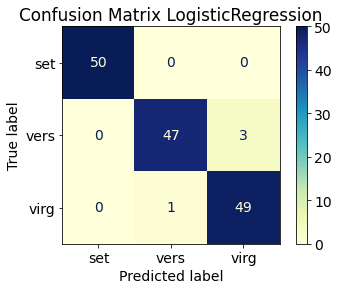
\includegraphics[width=0.23\linewidth]{Original_class/LogisticRegressionconfmat.png}}\\
		\subfloat{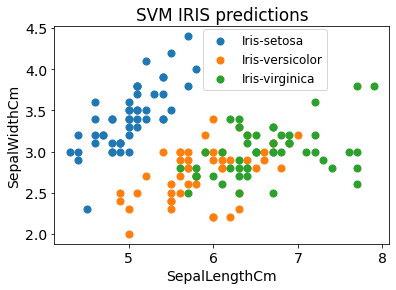
\includegraphics[width=0.26\linewidth]{Original_class/SVM IRIS predictions.png}}
		\subfloat{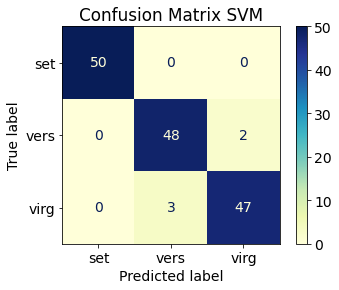
\includegraphics[width=0.23\linewidth]{Original_class/SVMconfmat.png}}
		\subfloat{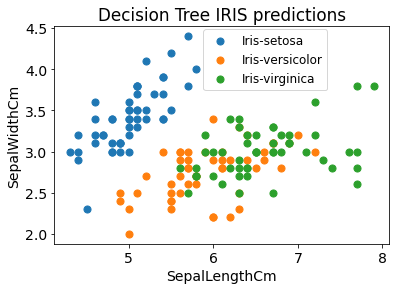
\includegraphics[width=0.26\linewidth]{Original_class/Decision Tree IRIS predictions.png}}
		\subfloat{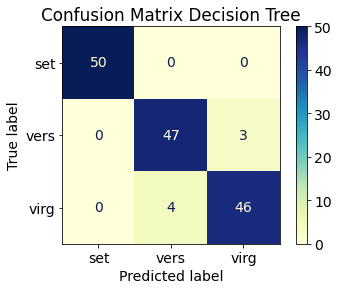
\includegraphics[width=0.23\linewidth]{Original_class/Decision Treeconfmat.png}}\\
		\subfloat{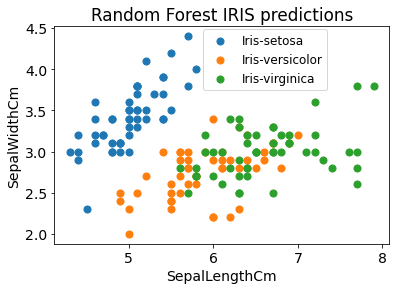
\includegraphics[width=0.26\linewidth]{Original_class/Random Forest IRIS predictions.png}}
		\subfloat{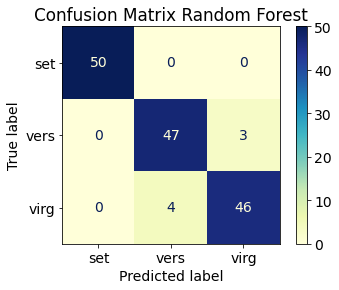
\includegraphics[width=0.23\linewidth]{Original_class/Random Forestconfmat.png}}
		\subfloat{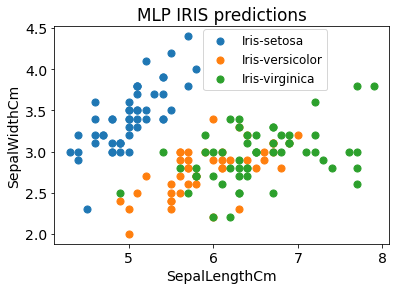
\includegraphics[width=0.26\linewidth]{Original_class/MLP IRIS predictions.png}}
		\subfloat{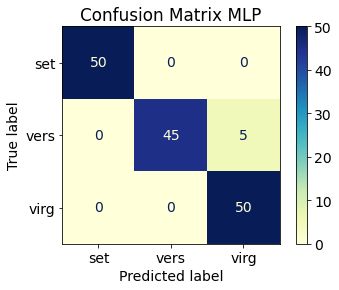
\includegraphics[width=0.23\linewidth]{Original_class/MLPconfmat.png}}
		\caption{Predikerte klynger og forvirringsmatriser for de forskjellige klassifikatorene på de originale Iris klyngene.}
		\label{fig:Orig_klynger}
	\end{figure*}
	
	
	\subsection{Klassifikator resultater}
	I Tabell~\ref{tab:Klassifikatorer} er accuracy (score) for de ulike klassifikatorene på de tre forskjellige klyngene, der 1 tilsvarer 100\% riktig gjetning sammenlignet med de sanne klassene. Predikert accuracy viser hvor likt KMeans~(Fig.~\ref{subfig:KMean_klynge}) og agglomerativ~(Fig.~\ref{subfig:Agglo_klynge}) metode lager klynger sammenlignet med de originale klassene~(Fig.~\ref{subfig:Orig_klynge}), m.a.o. samme som accuracy for forvirringsmatrisene i Figur~\ref{fig:Klynger_confmat}. Gjennomsnitt accuracy er over bare de seks klassifikatorene brukt.
	\begin{table}[h!]
		\centering
		%\hskip-2.5cm
		\begin{tabular}{| c | c | c | c |}
			\hline
			\rule{0pt}{10pt}Klynge & Original & Kmeans & Agglomerativ \\
			\hline
			\rule{0pt}{10pt}Predikert & - & 0.893 & 0.893 \\
			\hdashline
			\rule{0pt}{10pt}LR & 0.973 & 0.893 & 0.893 \\
			\rule{0pt}{10pt}KNN & 0.973 & 0.913 &  0.907 \\
			\rule{0pt}{10pt}SVM & 0.967 & 0.900 & 0.900 \\
			\rule{0pt}{10pt}DT & 0.953 & 0.893 & 0.907 \\
			\rule{0pt}{10pt}RF & 0.953 & 0.913 & 0.907 \\
			\rule{0pt}{10pt}MLP & 0.973 & 0.953 &  0.893 \\
			\hline
			\rule{0pt}{10pt}Gjennomsnitt & 0.965 & 0.911 & 0.901 \\
			\hline
		\end{tabular}
		\caption{Accuracy score for de ulike klassifikatorene på de tre forskjellige klyngene. Predikert accuracy viser hvor likt KMeans og agglomerativ metode lager klynger sammenlignet med de originale klassene.}
		\label{tab:Klassifikatorer}
	\end{table}
	
	
	\subsection{Klassifikator klyngeinndelinger}
	Figur~\ref{fig:Orig_klynger}-\ref{fig:Agglo_klynger} viser de predikerte resultatene med de ulike klassifikatorene på hver av de tre klyngene; original klynge~(Fig.~\ref{fig:Orig_klynger}), KMeans~(Fig.~\ref{fig:KMeans_klynger}) og agglomerativ~(Fig.~\ref{fig:Agglo_klynger}). For hver klassifikator er det vist de predikerte klyngene og tilhørende forvirringsmatrisene ved siden av hverandre. Egenskapkombinasjonen som er valgt for å vise de predikerte klyngene, er den samme som tidligere der noen av samplene til Iris-versicolor og Iris-virginica overlapper hverandre. Klassifikatorene er for hver av de tre klynge tilfellene trent på sin respektive klynge, men evaluert opp mot de sanne klassene i det originale Iris datasettet som har 50 sampler av hver klasse.
	
	\begin{figure*}[ht!]
		\vspace{-2.5cm}
		\centering
		\subfloat{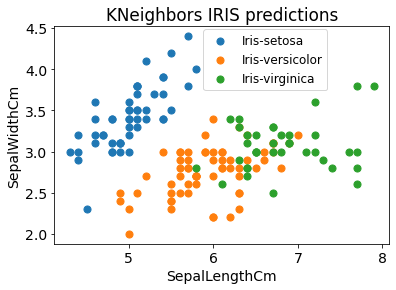
\includegraphics[width=0.26\linewidth]{KMeans_class/KMeansKNeighbors IRIS predictions.png}}
		\subfloat{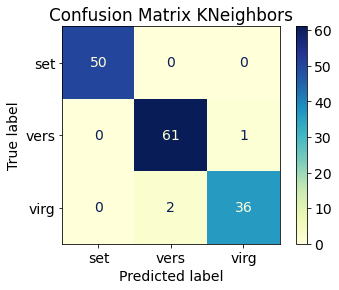
\includegraphics[width=0.23\linewidth]{KMeans_class/KMeansKNeighborsconfmat.png}}
		\subfloat{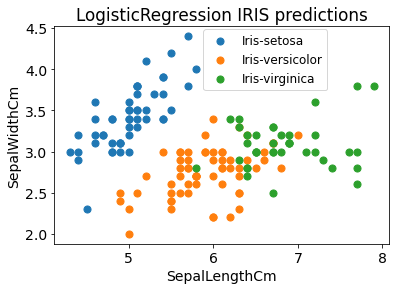
\includegraphics[width=0.26\linewidth]{KMeans_class/KMeansLogisticRegression IRIS predictions.png}}
		\subfloat{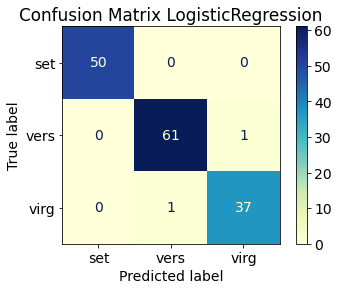
\includegraphics[width=0.23\linewidth]{KMeans_class/KMeansLogisticRegressionconfmat.png}}\\
		\subfloat{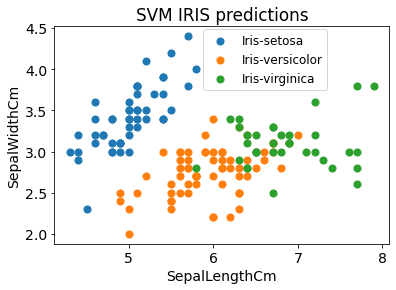
\includegraphics[width=0.26\linewidth]{KMeans_class/KMeansSVM IRIS predictions.png}}
		\subfloat{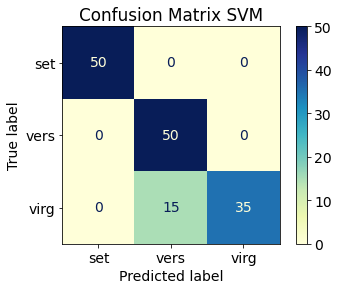
\includegraphics[width=0.23\linewidth]{KMeans_class/KMeansSVMconfmat.png}}
		\subfloat{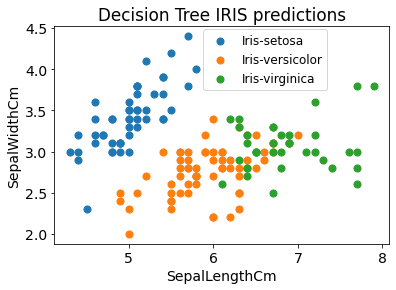
\includegraphics[width=0.26\linewidth]{KMeans_class/KMeansDecision Tree IRIS predictions.png}}
		\subfloat{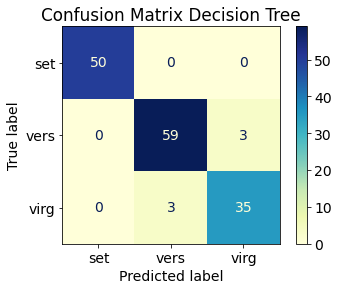
\includegraphics[width=0.23\linewidth]{KMeans_class/KMeansDecision Treeconfmat.png}}\\
		\subfloat{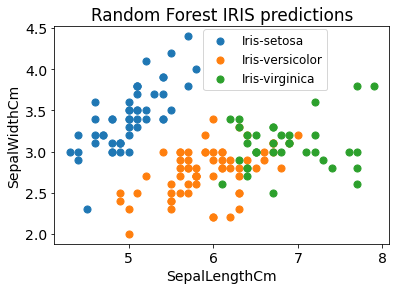
\includegraphics[width=0.26\linewidth]{KMeans_class/KMeansRandom Forest IRIS predictions.png}}
		\subfloat{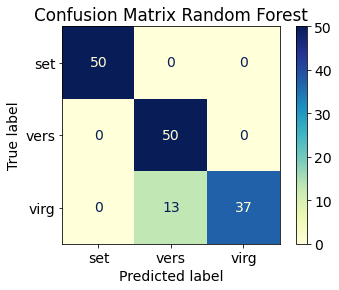
\includegraphics[width=0.23\linewidth]{KMeans_class/KMeansRandom Forestconfmat.png}}
		\subfloat{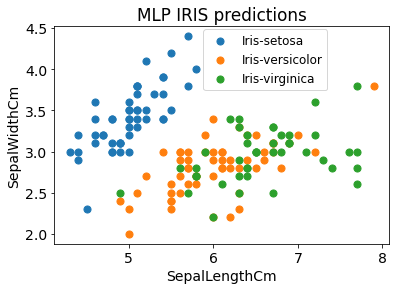
\includegraphics[width=0.26\linewidth]{KMeans_class/KMeansMLP IRIS predictions.png}}
		\subfloat{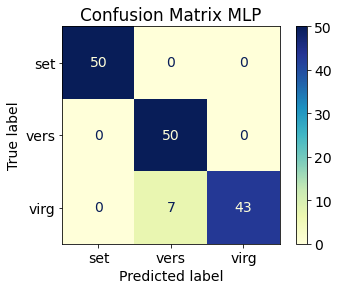
\includegraphics[width=0.23\linewidth]{KMeans_class/KMeansMLPconfmat.png}}
		\caption{Predikerte klynger og forvirringsmatriser for de forskjellige klassifikatorene trent på de predikerte KMeans klyngene.}
		\label{fig:KMeans_klynger}
	\end{figure*}
	
	\begin{figure*}[h!]
		\vspace{-0.83cm}
		\centering
		\subfloat{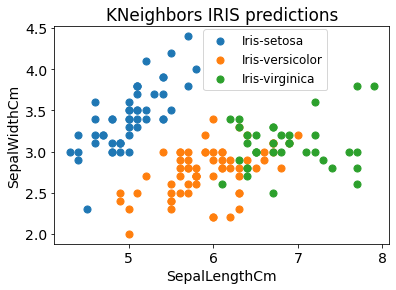
\includegraphics[width=0.26\linewidth]{Agglomerative_class/AggloKNeighbors IRIS predictions.png}}
		\subfloat{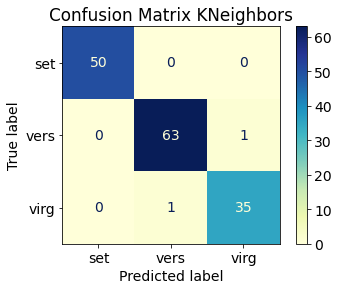
\includegraphics[width=0.23\linewidth]{Agglomerative_class/AggloKNeighborsconfmat.png}}			\subfloat{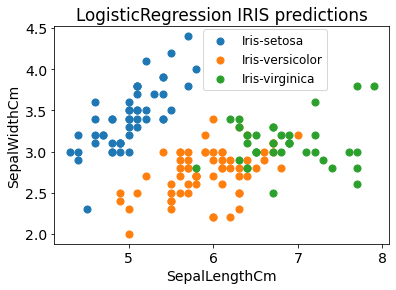
\includegraphics[width=0.26\linewidth]{Agglomerative_class/AggloLogisticRegression IRIS predictions.png}}
		\subfloat{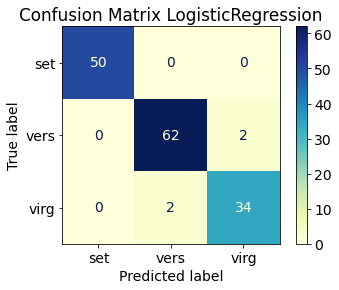
\includegraphics[width=0.23\linewidth]{Agglomerative_class/AggloLogisticRegressionconfmat.png}}\\
		\subfloat{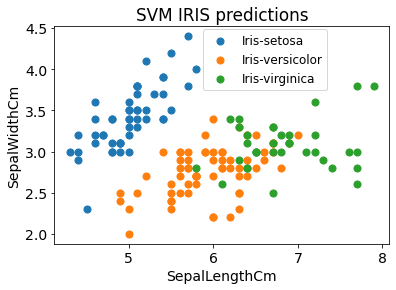
\includegraphics[width=0.26\linewidth]{Agglomerative_class/AggloSVM IRIS predictions.png}}
		\subfloat{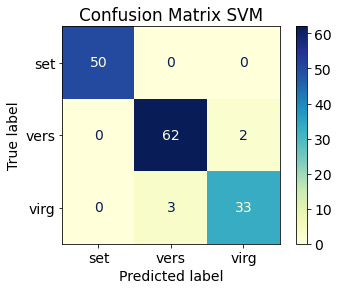
\includegraphics[width=0.23\linewidth]{Agglomerative_class/AggloSVMconfmat.png}}
		\subfloat{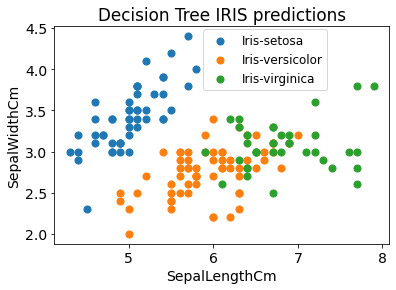
\includegraphics[width=0.26\linewidth]{Agglomerative_class/AggloDecision Tree IRIS predictions.png}}
		\subfloat{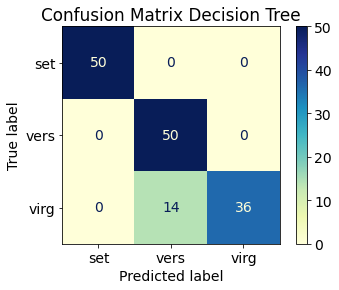
\includegraphics[width=0.23\linewidth]{Agglomerative_class/AggloDecision Treeconfmat.png}}\\
		\subfloat{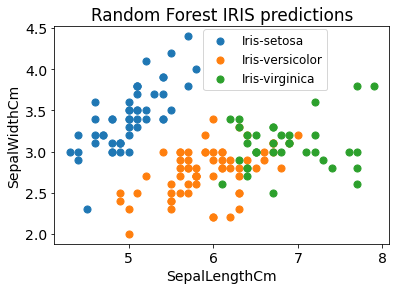
\includegraphics[width=0.26\linewidth]{Agglomerative_class/AggloRandom Forest IRIS predictions.png}}
		\subfloat{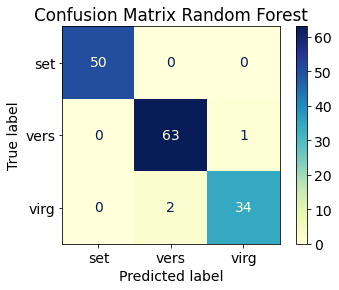
\includegraphics[width=0.23\linewidth]{Agglomerative_class/AggloRandom Forestconfmat.png}}
		\subfloat{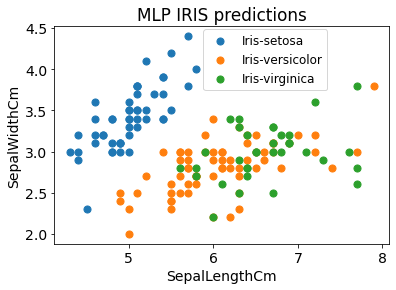
\includegraphics[width=0.26\linewidth]{Agglomerative_class/AggloMLP IRIS predictions.png}}
		\subfloat{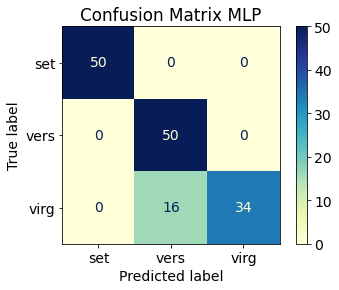
\includegraphics[width=0.23\linewidth]{Agglomerative_class/AggloMLPconfmat.png}}
		\caption{Predikerte klynger og forvirringsmatriser for de forskjellige klassifikatorene trent på de predikerte agglomerative klyngene.}
		\label{fig:Agglo_klynger}
	\end{figure*}
		
	
	\section{Diskusjon}
	I denne seksjonene blir resultatene og forskjeller på KMeans og agglomerativ metode diskutert.
	
	
	\subsection{Forskjeller på KMeans og Agglomerativ metode}
	Vanligvis pleier KMeans å være bra på store datasett fordi den er rask og enkel å implementere, og er ofte god til å balansere effektivitet og nøyaktighet. Den egner seg godt dersom det fins noe a prior kunnskap om datasettet, slik at det er en forståelse om hvor mange klynger datasettet skal deles inn i. For å bruke KMeans metoden så er nettopp en av input parameterne antall klynger datasettet skal deles i. I slike tilfeller er albue metoden god til å hjelpe å estimere hva antallet klynger kan være. KMeans metoden har en tendens til å favorisere sirkulære klynger, som ofte egner seg på datasett med global klynge form, og prøver å lage tette klynger.
	
	Sammenlignet med KMeans, er ikke den agglomerative metoden like godt egnet for store datasett på grunn av kompleksiteten i hvordan den lager klynger. Siden den lager et tre av mange klynger med utgangspunkt i antall klynger som antall sampler i datasettet, som reduseres til et gitt antall klynger eller til en stor felles klynge. Den trenger i tillegg å lage gode klynger i starten siden den kan ikke omgjøre valgene av å produsere tidligere klynger underveis, som kan lede til feil eller dårligere valg senere. Tilfellene der agglomerativ metode egner seg godt er for mindre datasett der det lønner seg å utforske forskjellig aspekter av data for å få finne strukturer som kan komme fram gjennom hierarkiske klynger. Klyngene behøver ikke ha like størrelser eller klynge former, og kan håndtere flere typer data.
	
	
	\subsection{Analyse av resultatene}
	%% Klynge dannelse
	Ved å sammenligne klyngene som produseres fra det originale Iris datasettet, KMeans og agglomerativ metode i Figur~\ref{fig:Datasett} og~\ref{fig:Pairplot}, så er det tydelig at det er mindre overlapp mellom Iris-versicolor og Iris-virginica samplene i KMeans og agglomerativ i forhold til det originale datasettet. Så det er tydelig at de to klynge-metodene skiller mer mellom versicolor og virginica samplene, som er naturlig siden de i utgangspunktet ikke har tilgang til de sanne klasse når de lager de nye klyngene. Måten de lager de nye klyngene på er å samle likere sampler sammen. Så når det er overlapp mellom noen av sample-egenskapene i forskjellige klasser, så vil det også være noen prediksjoner som blir forskjellige siden de setter samplene til den nærmeste klynge senteret.
	
	%% Klynge metode inndelingene
	Rent visuelt så er det ikke stor forskjell mellom KMeans og agglomerativ klyngene, det er noen versicolor og virginica sampler som er litt forskjellige i overlapp områdene mellom de to klyngene i Figur~\ref{fig:Datasett} og~\ref{fig:Pairplot}. For å se nærmere på prediksjonene av samplene, så vises det hva KMeans og agglomerativ predikerer riktig og feil i forvirringsmatrisen i Figur~\ref{fig:Klynger_confmat}. Der kommer det mer tydelig fram hva de to metodene predikerer, og i utgangspunktet så er det 50 sampler av hver klasse i det originale datasettet. Begge metodene predikerer flere versicolor sampler enn virginica sampler. Istedenfor 50 av hver så er det i de nye klyngene 62 og 64 versicolor sampler. Iris-setosa samplene har egenskaper som er så ulike de to andre klassene, slik at de alltid er mye lettere å gruppere og predikere riktig. Men totalt så har de begge en accuracy score på 0.893 (Se Tabell~\ref{tab:Klassifikatorer}), så de er totalt sett like gode.
	
	%% Klassifikasjons resultatene
	Av klassifikatorene som lærer og predikerer på det originale datasettet, så er det LR, KNN og MLP klassifikatorene som er best med accuracy på 0.973. Alle klassifikatorene har accuracy over 0.95, som er ganske bra på dette datasettet. Ingen av klassifikatorene har blitt optimalisert med hensyn på modell parametre, men kun brukt for å vise forskjeller med enkle, ofte brukte klassifikatorer. Det samme gjelder på KMeans og agglomerativ klyngene.
	
	%KMeans og Agglo
	For å evaluere KMeans og agglomerativ klyngene, så er disse klyngene ikke like det originale datasettet, siden de har predikert nye klasser slik at det ikke lenger er 50 sampler av alle tre klassene, som vist i Figur~\ref{fig:Klynger_confmat}. Dette vil da ha noe å si for hvordan klassifikatorene trener på de to predikerte klynge-settene. Dette synes ved å se på accuracy score i Tabell~\ref{tab:Klassifikatorer}, der klassifikatorene presterer bedre på det originale datasettet enn på de to predikerte klynge-metodene. Dette kommer fra de tilfellene der egenskapene til noen av versicolor og virgincia samplene overlapper hverandre, slik at KMeans og agglomerativ predikerer feil klasse på noen sampler. Klassifikatorene klarer da ikke å predikere disse riktig i forhold til de sanne klassene, som senker accuracy noe. 
	
	Mellom KMeans og agglomerativ, så presterer klassifikatorene gjennomsnittlig litt bedre når de er trent på KMeans, 0.911 mot 0.901 med agglomerativ. Det er ikke mye forskjell, og hovedforskjellen mellom dem er hvordan MLP klassifikatorene presterer. For de andre klassifikatorene er accuracy mye likere, mens med MLP er det 0.953 mot 0.893. Denne forskjellen kan være på grunn av tilfeldigheter, siden prestasjonene vil avhenge av tilfeldigheter i både trening og i klassifikatorene som kan endre seg hver gang programmet i Python kjøres. Men kan være andre grunner.
	
	Setosa samplene blir alltid predikert riktig, uansett hvilken klassifikator som er brukt. Dette kommer av at disse samplene har ulike nok egenskaper i forhold til de to andre klassene, at det er lett å skille denne klassen fra de to andre. For forvirringsmatrisene i Figur~\ref{fig:Orig_klynger}, så er det ganske lik fordeling av predikerte feil mellom versicolor og virginica klassene. For KMeans og agglomerativ så er det hovedsaklig overtall av predikerte feil der noen virginica sampler er klassifisert som versiocolor. Dette kommer mest sannsynlig av at KMeans og agglomerativ begge lager klynger der virginica sampler blir satt i klynger med versicolor sampler utifra noen like egenskaper, som igjen klassifikatorene lærer seg og predikerer feil mot de sanne klassene. Dette blir og mer tydelig vist i Figur~\ref{fig:Pairplot}, ved å sammenligne den øverste figuren med klynger for de originale egenskapkombinasjonene mot de to andre under, for KMeans og agglomerativ. For de to predikerte så er det ofte flere oransje versicolor prikker i forhold til grønne virginica prikker enn det er for de originale kombinasjonene. De predikerte klyngene har tydeligere mindre overlapp mellom versicolor og virginica sampler.
	
	Totalt sett så går prestasjonene litt ned for klassifikatorene når de trenes med klyngemetodene, men ikke med mye. Alle gjennomsnittene for de tre klyngene er over 0.9, som ofte regnes som bra resultater i klassifisering. Dette er i tillegg med at de sanne klassene er kjente, som ofte ikke er tilgjengelige i tilfeller det brukes klyngemetoder. Så klyngemetoder kan ofte være veldig gode på å gruppere sampler sammen i klynger som kan tilnærmes som klasser for opptrening av klassifikatorer og videre analyse.


	\section{Konklusjon}
	Klyngeanalyse brukes ofte i ikke-ledet læring tilfeller der vi har sampler fra flere ukjente klasser i et datasett. Forskjellige klyngemetoder, som KMeans og agglomerativ metode, kan brukes for å tilegne samplene inn i like klynger etter egenskapene til samplene. Disse inndelte klyngene kan brukes til å trene opp f.eks. klassifikatorer utifra klasseinndelingen/klyngene til klyngemetodene.
	
	Det originale datasettet er best å bruke, og gir høyere predikert accuracy for de brukte klassifikatorene. Men ofte så er det ikke sikkert at de sanne klassene er tilgjengelige i datasett. Så klyngemetoder, som har blitt brukt her, viser at på Iris datasettet så er det en liten nedgang i hvor nøyaktige klassifikatorene blir, men klyngemetodene viser at det ikke er stor forskjell slik at de fint kan brukes for å tildele ukjente sampler inn i klynger/klasser som er i nærheten av de sanne klassene. Det kan ofte og være ekstra informasjon å få ved å gjøre klyngeanalyse.
	
	
	\appendix
	\section{Python kode}
	\label{Appendix:Kode}
	Koden og resultater som er brukt i dette prosjektet kan bli funnet i GitHub på: \url{https://github.com/krilangs/TEK9020/tree/main/Project3}
	
\end{document}
